\documentclass[11pt,a4paper]{article}

\usepackage[utf8]{inputenc}
\usepackage[english]{babel}
\usepackage[T1]{fontenc}
\usepackage{graphicx}


\usepackage{amsmath,amssymb,amsfonts}

\title{Assignment 1}
\author{Sebastian Paaske Tørholm \& Kristoffer Søholm}

\begin{document}
\maketitle

\section{Question 1.1}
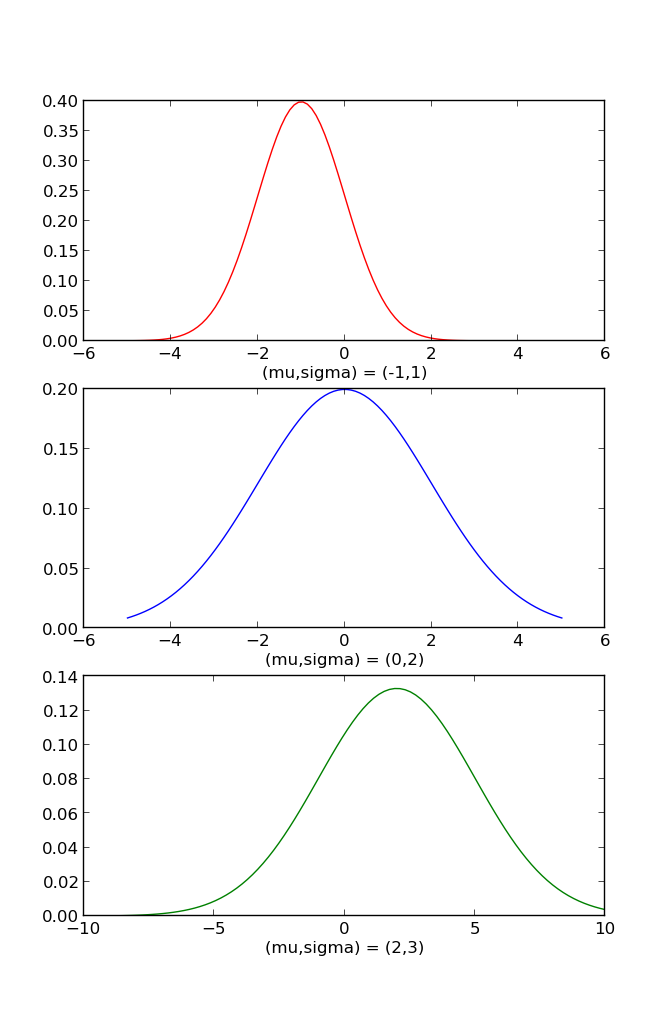
\includegraphics[scale=0.6]{figure_1.png}
\section{Question 1.2}
See the attached source.
\section{Question 1.3}
We see a deviation from the correct mean due to the values being randomly sampled. Thus it
is unlikely that we get an exact match between the sample mean and the correct mean.

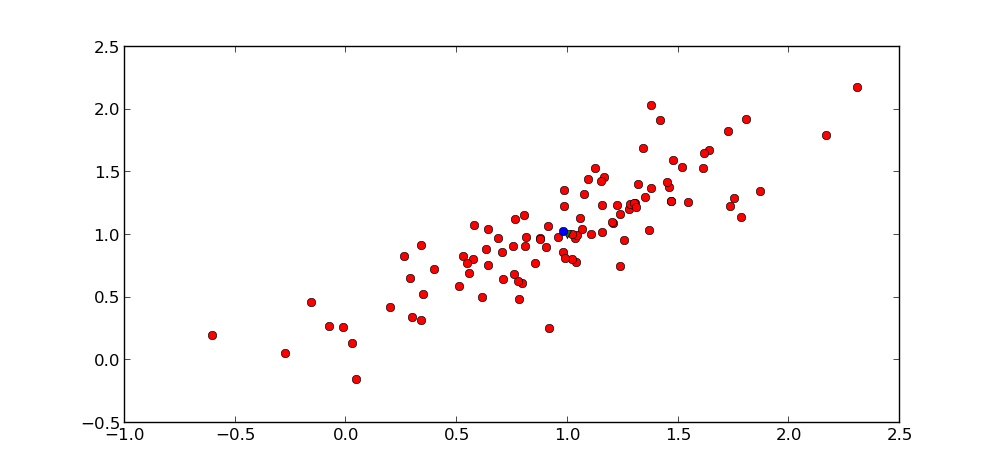
\includegraphics[scale=0.6]{figure_2.png}
\section{Question 1.4}
In order to marginalize $x_c$ out, it is sufficient to simply drop the parts of $x$, $\mu$, and $\Sigma$ which contains subscript c's. 
\section{Question 1.5}
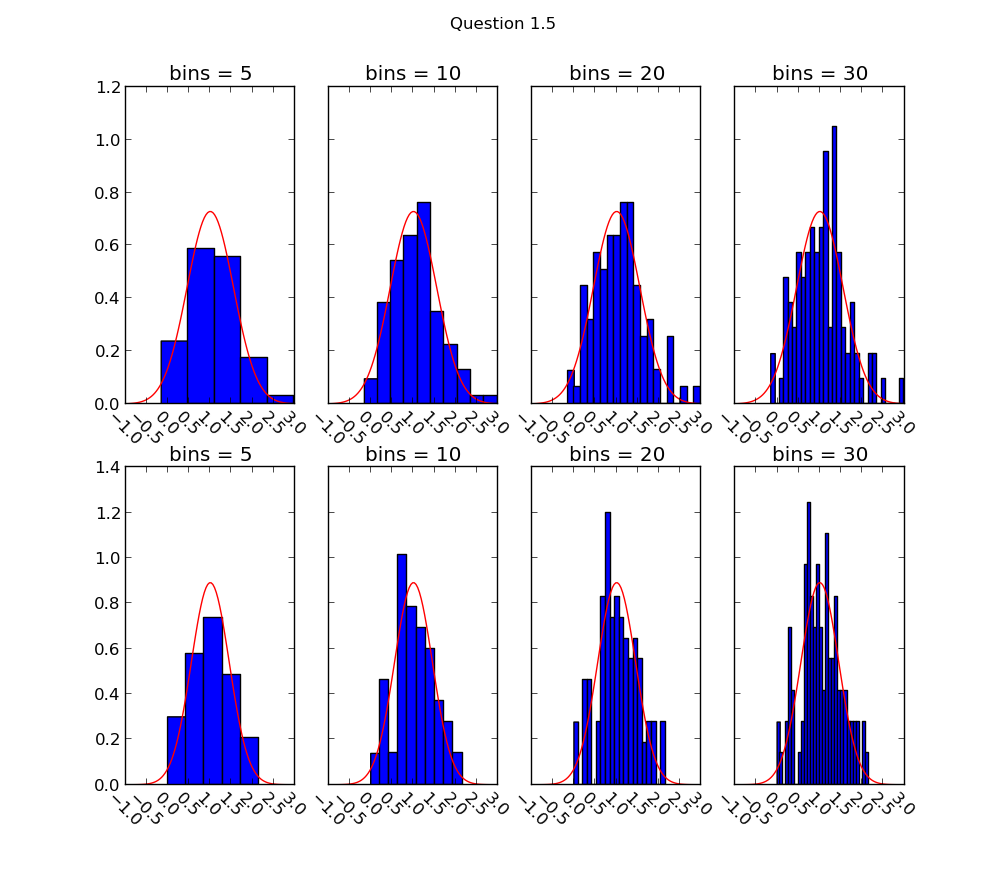
\includegraphics[scale=0.6]{figure_3.png}

Increasing the number of bins makes the histogram more accurate up to a point. As can be seen from the examples with 30 bins, the histogram becomes more erratic, as two adjacent bins get very different heights due to random fluctutations.
\section{Question 1.6}
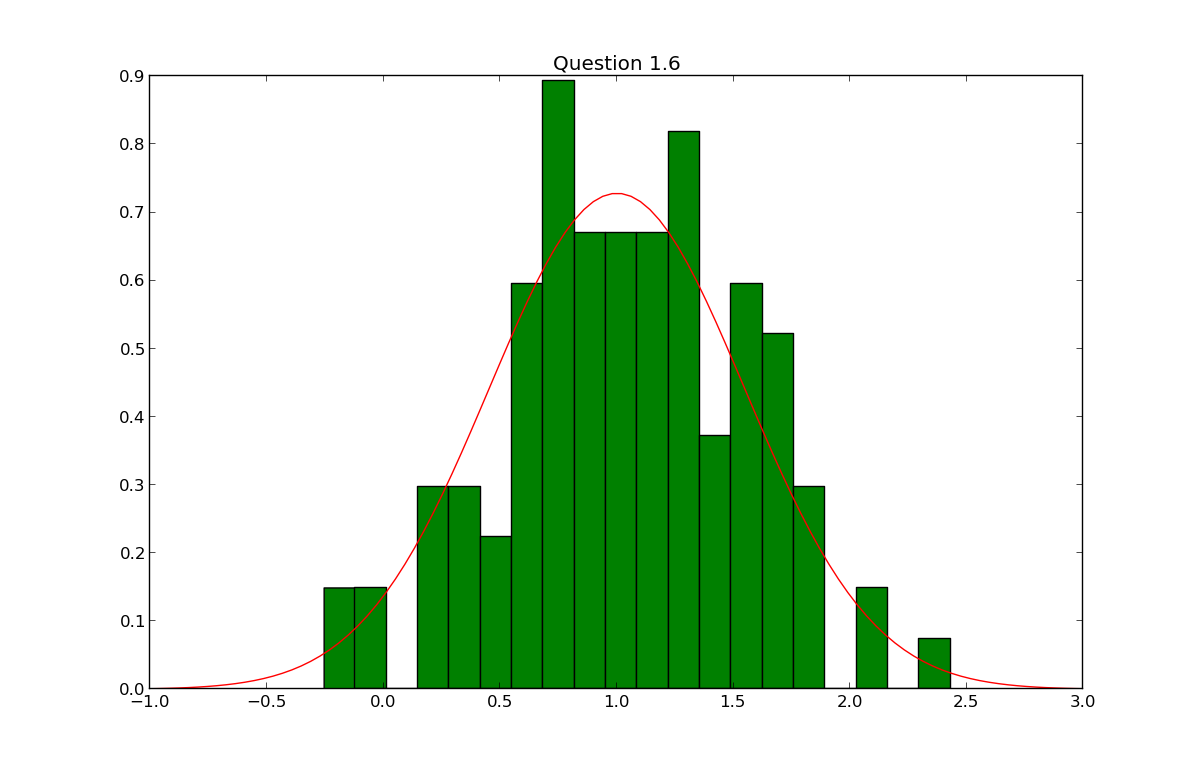
\includegraphics[scale=0.5]{figure_4.png}

The analytical expression for the marginal distribution $p(x_1)$ is given by:

$$ p(x_1) = \mathcal{N}(x_1 | 1, 0.3) $$
\section{Question 1.7}
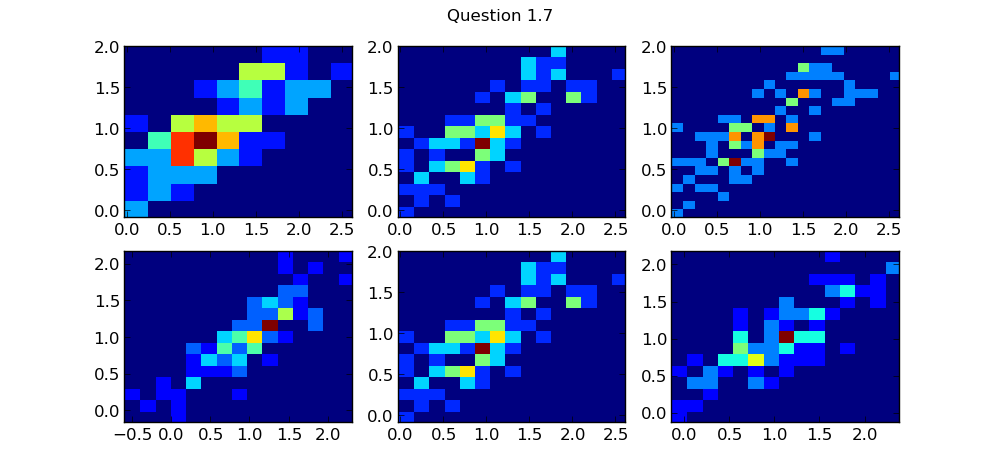
\includegraphics[scale=0.6]{figure_5.png}
\section{Question 1.8}
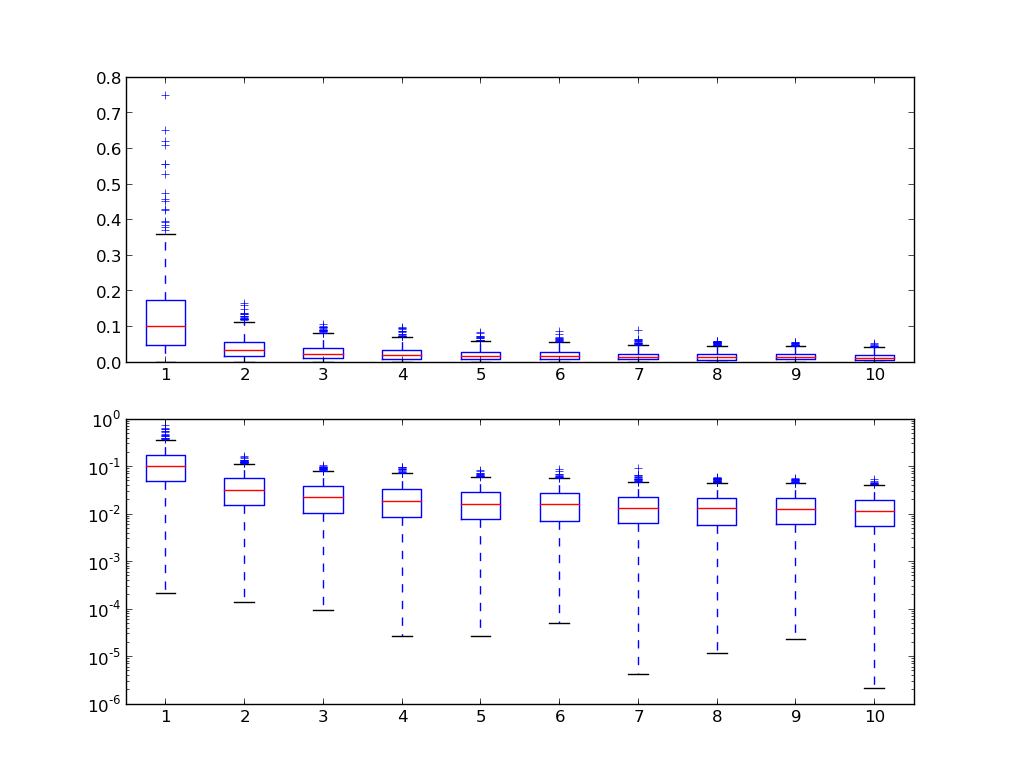
\includegraphics[scale=0.6]{figure_6.png}
\section{Question 1.9}
\section{Question 1.10}
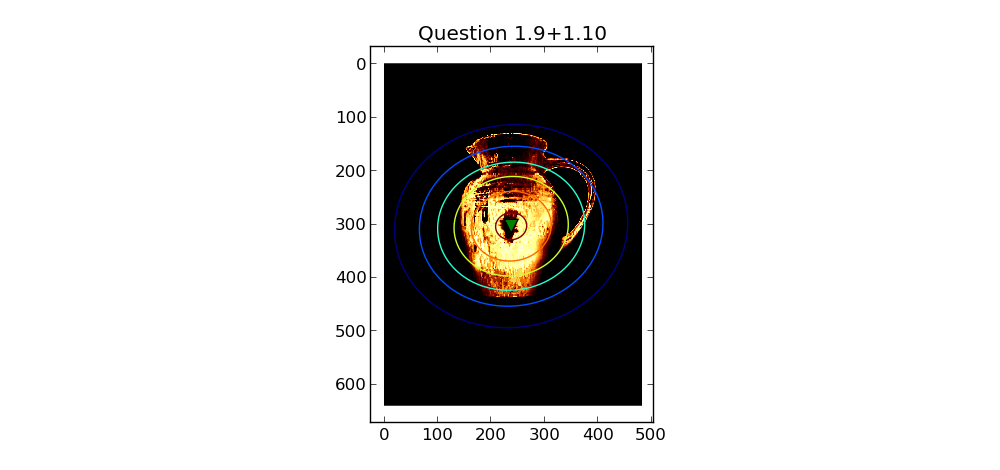
\includegraphics[scale=0.6]{figure_8.png}
\section{Question 1.11}
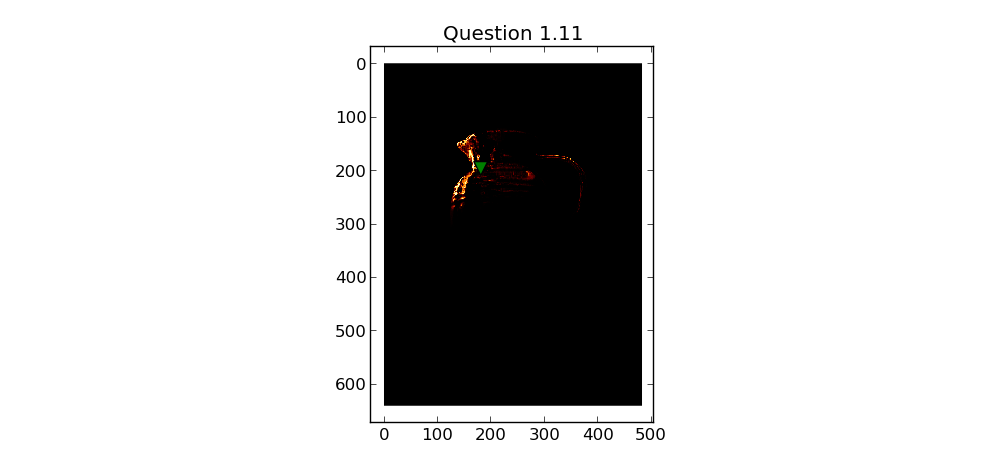
\includegraphics[scale=0.6]{figure_9.png}

\end{document}

